
\documentclass[10pt]{article}

\usepackage[utf8]{inputenc}
\usepackage{xcolor}
\usepackage{float}
\usepackage{graphicx}
\usepackage{geometry}
\usepackage{float}
\usepackage[toc,page]{appendix}
\graphicspath{ {./images/} }
\parindent=0pt
\usepackage{hyperref}
\hypersetup{
    colorlinks = true,
    linkcolor = blue,
    citecolor=blue,
    linkbordercolor = {white},
}
\usepackage{fullpage}
\usepackage{fancyvrb}

\frenchspacing

\usepackage{microtype}

\usepackage[english,dutch]{babel}

\usepackage{listings}
% Er zijn talloze parameters ...
\lstdefinestyle{myStyle}{
    belowcaptionskip=1\baselineskip,
    breaklines=true,
    frame=none,
    numbers=left, numberstyle=\tiny, numberfirstline=false, breaklines=true,
    stepnumber=1, tabsize=8,
    basicstyle=\footnotesize\ttfamily,
    keywordstyle=\bfseries\color{blue!40!black},
    commentstyle=\itshape\color{green!40!black},
    identifierstyle=\color{black},
}

\title{Opdracht 3}
\author{Jenny Vermeltfoort}

\begin{document}

\selectlanguage{dutch}
\def\tablename{Tabel}

\maketitle

\section{Uitleg}
Dit verslag beschrijft een applicatie die een cellulaire automaat, specifiek, \textit{Life} ontwikkeld door John Horton
Conway, implementeert \cite{martin-garder}. \textit{Life} is een 2d wereld waarin leven wordt gesimuleerd. Deze wereld
wordt gelimiteerd door een aantal regels; wanneer een dode cel drie levende buren heeft komt de dode cel tot leven; een
levende cel sterft wanneer er minder als twee of meer als drie buurtgenoten in haar omgeving zijn. Buurtgenoten zijn de
8 cellen die direct diagonaal, horizontaal, en verticaal, de aangewezen cel raakt. De gebruiker van de applicatie heeft
bepaalde controle over de wereld, zie de lijst verder in deze sectie. Met bepaalde configuraties zijn ongelofelijk
prachtige generaties te maken, zie bijvoorbeeld de oscillator in figuur \ref{fig:kok}.

\hfill
\begin{figure}[H]
    \centering
    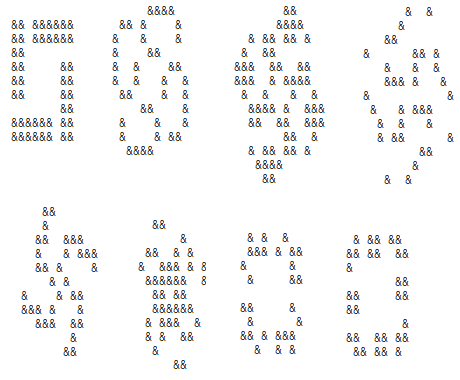
\includegraphics[width=0.6\linewidth]{ga_all}
    \caption{Kok's Galaxy oscillator\cite{galaxy-blog}. }
    \label{fig:kok}
\end{figure}
\hfill

De gebruiker van de applicatie kan het volgende:
\begin{enumerate}
    \item het programma stoppen,
    \item het aantal generaties beheren, inclusief een oneindige hoeveelheid generaties,
    \item doormiddel van een cursor cellen tot leven of tot steven brengen,
    \item de wereld of view met een configureerbare aantal random gelokaliseerde cellen vullen,
    \item bepalen welke karakters levende, dode, of rand karakters worden gepresenteerd,
    \item de view verplaatsen met een configureerbare aantal stappen,
    \item de refresh rate bepalen wanneer de applicatie oneindig doorloopt.
\end{enumerate}

\section{Implementatie}
De wereld bestaat uit twee 2d matrices, een matrix die de boolean waarde van een cel beschrijft en een matrix die het
bijbehorende karakter van de cel beschrijft. Deze twee matrices liggen langs elkaar in het geheugen. Hierdoor kan er
met een pointer naar een cel in de boolean matrix, de pointer naar een cel in de karakter matrix worden berekend met
\verb|char_ptr = bool_ptr + size_matrix.x|. De reden hiervoor is om de generatie loop zo efficiënt mogelijk te maken,
voornamelijk de functie \verb|World::world_valide_cells| en de functie \verb|View::refresh_view|. Met een aantal
optimalisatie methodes is de generatie loop van ongeveer 71 msec per generatie naar ongeveer 5 msec gegaan. Getest
op dezelfde PC, zonder optimalisatie van de compiler.

Het berekenen van het aantal levende buurtgenoten moet voor elke cel in de wereld gedaan worden voor een
generatie. Het is daarmee van belang om deze berekening zo te implementeren dat deze het minst aantal CPU cycles
uitvoert. Dit is mogelijk door minder instructies uit te voeren of door bepaalde instructies te vervangen door
`\textit{cycle-friendly}` instructies.

De levende wereld is daarmee zo ingericht dat de randen van de matrixen doden cellen
bevatten, de levende wereld bestaat dus uit een matrix met coördinaten	(1,1) tot (world\_size.x -1, world\_size.y -
1).
Hierdoor hoeft er niet gecontroleerd te worden of de buren van een cel buiten de matrix vallen.

Verder is doorgaans de selectie van een 2d matrix in c++ enigszins  inefficiënt, notatie \verb|cell = world[y][x]|. Dit
komt omdat voor elke cel selectie met deze methode een \verb|mul| instructie uitvoert; berekening \verb|cell =|
\verb|ptr + y * size.x + x|. Deze multiplication instructie
kost meer CPU cycles dan een addition instructie\cite{cpu-cost-instructions}. Door de cellen te vinden met pointers is
het mogelijk om de multiplicatie instructie te verwijderen.

Zie een stuk code uit de functie \verb|World::world_valide_cells| beneden voor context en als voorbeeld.
\begin{verbatim}
    for (y = limit_y; y > 0; y--) {
        for (x = limit_x; x > 0; x--) {
            count = (*(cell_ptr - world_size.x - 1) +
                     *(cell_ptr - world_size.x)) +
                    (*(cell_ptr - world_size.x + 1) +
                     *(cell_ptr - 1)) +
                    (*(cell_ptr + 1) +
                     *(cell_ptr + world_size.x - 1)) +
                    (*(cell_ptr + world_size.x) +
                     *(cell_ptr + world_size.x +
                       1));

            if ((*cell_ptr && count != 2 && count != 3) ||
                (!*cell_ptr && count == 3)) {
                event_add(cell_ptr);  // an event toggles the
                                      // cell' value. !note: this function is inlined.
            }
            cell_ptr++;
        }
        cell_ptr += 2;  // skip border right on y and left on y+1
    }
\end{verbatim}

Een event is in deze context slechts een pointer naar een cel die geschakeld moet worden, deze
lijst van pointers wordt later in de generatie loop verwerkt. Aangezien \textit{branching} kostbaar is, voornamelijk
wanneer de
CPU een verkeerde branch gist, is het van belang om de
\verb|if| statement in de stuk code niet te branchen\cite{cpu-cost-instructions}. Hiervoor is het noodzakelijk dat een
\verb|event| de cel waarde schakelt, in plaats van dat een event de cel met een gespecificeerde
waarde vult.

\section{Gebruik}
Zorg er ten eerste voor dat er een \verb|./glidergun.txt| in dezelfde folder staat als de applicatie. De volgende
inputs kunnen door de gebruiker geleverd worden:
\begin{small}
    \begin{verbatim}
    See the list below for all options, input is parsed after each <enter>.
    Usage example: 'pca@\n' sets the alive cell representation to '@'.
    <h>                    this help.
    <e>                    stop the programm.
    <g><a/s>               generations sub-menu.
      <a>                  toggle auto run mode.
      <s>[num]             when in run_mode = '0', perform [num] amount of generations.
    <r>                    reset the view.
    <8,6,4,5>              move the view left(4), right(6), top(8), bottom(5) by configured step size, see <p><v>.
    <w,a,s,d>              move the the cursor left(a), right(d), top(w), bottom(s).
    <t>                    toggle the cell highlighted by the cursor (pink).
    <i><v/v[num]/w/w[num]> infest sub-menu.
      <v>                  randomly infest the view with default infest cell count, see <p><i><v>.
      <v>[num]             randomly infest the view with [num] amount of cells.
      <w>                  randomly infest the world with default infest cell count, see <p><i><w>.
      <v>[num]             randomly infest the world with [num] amount of cells.
    <p><c/i/v/r/s>         parameter sub-menu.
      <c><a/d/b>           cell sub-menu.
        <a>[char]          set alive cell representation to [char], example: 'pca@'.
        <d>[char]          set dead cell representation to [char].
        <b>[char]          set border cell representation to [char].
      <i><v/w>             infest sub-menu.
        <v>[num]           set default infest cell count to [num], view, see <i><v>.
        <w>[num]           set default infest cell count to [num], world, see <i><w>.
      <v><y/x>             view sub-menu
        <y>[num]           set view move step size, y axis, see <8,6,4,5>.
        <x>[num]           set view move step size, x axis, see <8,6,4,5>.
      <r>[num]             set the refresh rate to [num] milliseconds, example 'pr100'.
      <s>[num1];[num2]     set view size to y = num1, x = num2.
\end{verbatim}
\end{small}

\section{Tijd}
Zie tabel \ref{tab:time} voor de tijd verantwoording.

\begin{table}[H]
    \begin{center}
        \begin{tabular}{ l c }
            Week & Uur \\ \hline
            42   & 8   \\
            43   & 4   \\
            45   & 8   \\
        \end{tabular}

        \caption{Tijd verantwoording}
        \label{tab:time}
    \end{center}
\end{table}

\bibliographystyle{ieeetr}
\bibliography{bibtex.bib}

\newgeometry{left=2cm,bottom=2cm,top=2cm, right=2cm}
\newpage
\begin{appendices}
    \section{Code}\label{sec:code}
    \lstinputlisting[caption=main.cpp,
        label={lst:listing-cpp},
        language=C++,
        style=myStyle]{../src/main.cc}
\end{appendices}

\end{document}